%%%%%%%%%%%%%%%%%%%%%%%%%%%%%%%%%%%%%%%%%%%%%%%%%%%
%% P3: Phenomenology of Particle Physics                         
%%
%% Author:  André Rubbia                   		 
%%
%% Figure 11.18 The kinematics of the Compton process in the laboratory frame.
%%
%% This work is licensed under the Creative Commons Attribution 4.0 International License. 
%% To view a copy of this license, visit http://creativecommons.org/licenses/by/4.0/ or 
%% send a letter to Creative Commons, PO Box 1866, Mountain View, CA 94042, USA.
%%
%%%%%%%%%%%%%%%%%%%%%%%%%%%%%%%%%%%%%%%%%%%%%%%%%%%

\documentclass[a4paper,10pt]{article}

\usepackage[T1]{fontenc}
\usepackage[utf8]{inputenc}
\usepackage{lmodern}
\usepackage[labelfont=bf]{caption}
\usepackage{upgreek}

\usepackage{tikz}
\usepackage{pgfplots}
\pgfplotsset{compat=1.17}
\usepgfplotslibrary{ternary}
\usepgfplotslibrary{fillbetween}
\usepgfplotslibrary{external}

\usepackage{braket}

\def\d{\mathrm{d}}

\begin{document}

%%%%%%%%%%%%%%%%% FIGURE %%%%%%%%%%%%%%%%%%%%%%%%%%%%%%%%%%
\begin{figure}[htb]
\begin{center}
\mbox{
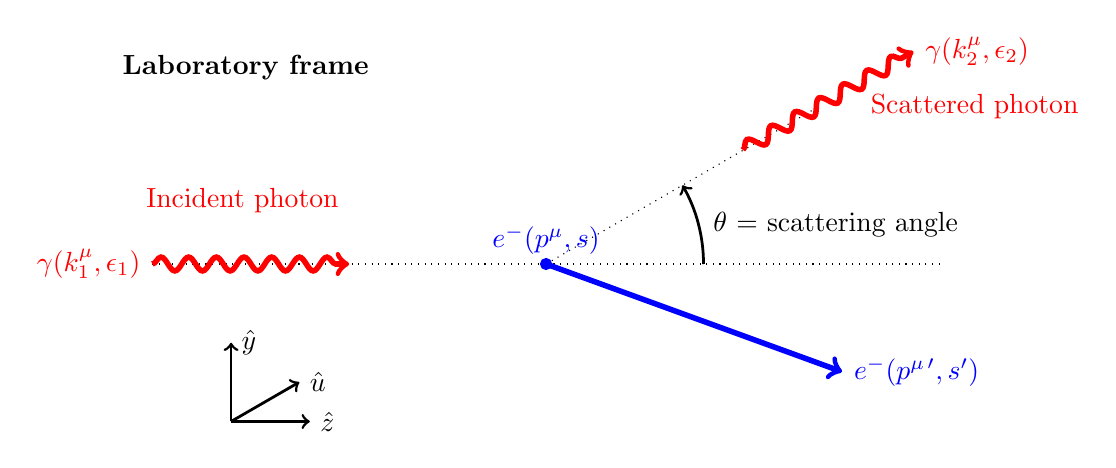
\begin{tikzpicture}
\draw[dotted] (-5,0)  -- (0,0);
\draw[dotted] (5,0)  -- (0,0);
\draw[dotted] (0,0) -- +(30:4);
\draw[thick,->,line width=1pt] (2,0) arc [radius=2, start angle =0, end angle=30];
\draw (2,0.5) node[right] {$\theta$ = scattering angle};
\draw[->,line width=1pt] (-4,-2) -- (-3,-2) node[right] {$\hat z$};
\draw[->,line width=1pt] (-4,-2) -- (-4,-1) node[right] {$\hat y$};
\draw[->,line width=1pt] (-4,-2) -- +(30:1) node[right] {$\hat u$};
\draw[red,line width=2pt,->,decorate, decoration=snake] (-5,0)  node[left] {$\gamma(k^\mu_1,\epsilon_1)$} -- (-2.5,0);
\draw[red, line width=2pt, ->,decorate, decoration=snake] (2.5,1.45)  -- +(30:2.5) node[right] {$\gamma(k^\mu_2,\epsilon_2)$};
\filldraw [blue] (0,0) circle (2pt) node[above] {$e^-(p^\mu,s)$};
\draw[blue, ->,line width=2pt] (0,0)  -- +(-20:4) node[right] {$e^-(p^{\mu\, \prime},s')$} ;
\draw[] (-5.5,2.5) node[right] {\textbf{Laboratory frame}};
\draw[red] (-5.2,0.8) node[right] {Incident photon};
\draw[red] (4,2) node[right] {Scattered photon};
\end{tikzpicture}
}
\caption{The kinematics of the Compton process in the laboratory frame. }
\end{center}
\end{figure}
%%%%%%%%%%%%%%%%% END FIGURE %%%%%%%%%%%%%%%%%%%%%%%%%%%%%%
%

\end{document}
